\begin{figure}[H]
    \centering
    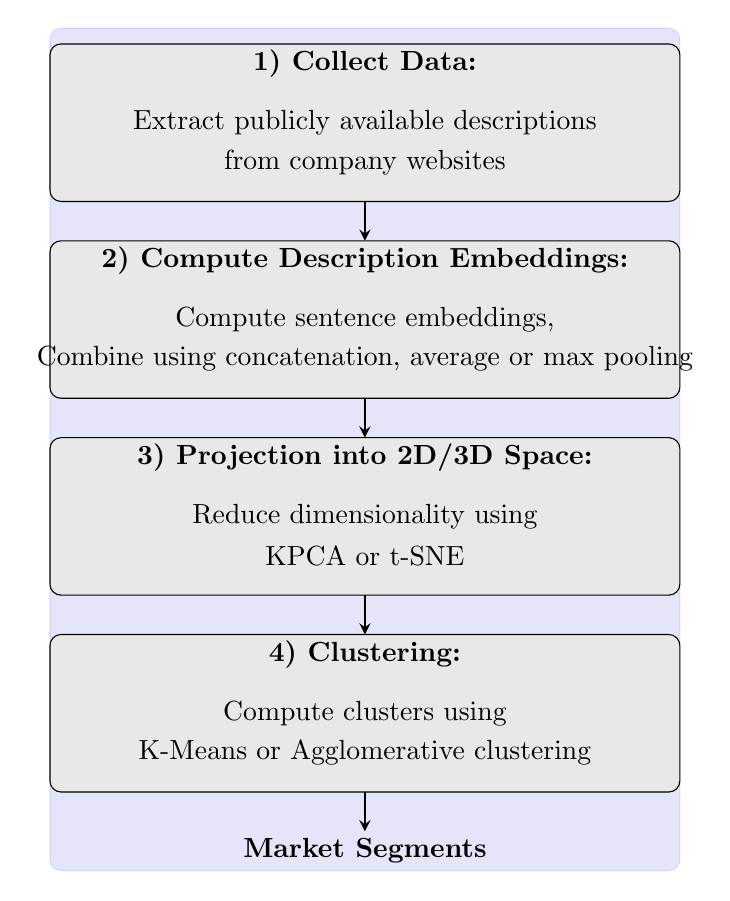
\begin{tikzpicture}
        \definecolor{lightgrey}{RGB}{232,232,232}
        \definecolor{darkblue}{RGB}{0,0,204}
        
        \draw[rounded corners, darkblue, fill=darkblue, opacity=0.1] (-4, -1) rectangle (4, 9.7);
    
        \draw[rounded corners, fill=lightgrey] (-4,7.5) rectangle (4, 9.5);
        \node[font=\bfseries] at (0, 9.25) {1) Collect Data:};
        \node at (0, 8.5) {Extract publicly available descriptions};
        \node at (0, 8.0) {from company websites};
        \draw[thick, -stealth] (0, 7.5) -- (0, 7);
    
        \draw[rounded corners, fill=lightgrey] (-4,5) rectangle (4, 7);
        \node[font=\bfseries] at (0, 6.75) {2) Compute Description Embeddings:};
        \node at (0, 6) {Compute sentence embeddings,};
        \node at (0, 5.5) {Combine using concatenation, average or max pooling};
        \draw[thick, -stealth] (0, 5) -- (0, 4.5);

        \draw[rounded corners, fill=lightgrey] (-4,2.5) rectangle (4, 4.5);
        \node[font=\bfseries] at (0, 4.25) {3) Projection into 2D/3D Space:};
        \node at (0, 3.5) {Reduce dimensionality using};
        \node at (0, 3.0) {KPCA or t-SNE};
        \draw[thick, -stealth] (0, 2.5) -- (0, 2);

        
        \draw[rounded corners, fill=lightgrey] (-4,0) rectangle (4, 2);
        \node[font=\bfseries] at (0, 1.75) {4) Clustering:};
        \node at (0, 1) {Compute clusters using};
        \node at (0, 0.5) {K-Means or Agglomerative clustering};
        \draw[thick, -stealth] (0, 0) -- (0, -0.5); 

        \node[font=\bfseries] at (0, -0.75) {Market Segments};
    \end{tikzpicture}
    \caption{Overview of our clustering pipeline.}
    \label{fig:pipeline}
\end{figure}
\pe{ s/Market Segments/Local Clusters; Market segment seems to be defined as segmenting your customer base \href{https://en.wikipedia.org/wiki/Market_segmentation}{wiki market segmentation}}

